%%%%%%%%%%%%%%%%%%%%%%%%%%%%%%%%%
% 6CCS3PRJ Final Year Individual Project Report
% zafira.shah@kcl.ac.uk
%%%%%%%%%%%%%%%%%%%%%%%%%%%%%%%%%
\documentclass[11pt]{informatics-report}
\usepackage{color}
\usepackage[square,sort,comma,numbers]{natbib} %References
\usepackage{xcolor}
\usepackage{listings}
\usepackage{pythonhighlight}
\usepackage{xparse}
\usepackage{float}



%%%%%%%%%%%%%%%%%%%%%%%%%%%%%%%%%
% Front Matter - project title, name, supervisor name and date
%%%%%%%%%%%%%%%%%%%%%%%%%%%%%%%%%
\title{6CCS3PRJ Final Year Project\\\vspace{0.2cm}Adafruit CLUE (Development Board)}
\author{Zafira Shah}
\studentID{19008701}
\supervisor{Dr Jeffery Raphael}

\date{\today}

\abstractFile{FrontMatter/abstract.tex}
\ackFile{FrontMatter/acknowledgements.tex} %Remove line if you do not want acknowledgements

\begin{document}
\createFrontMatter
\onehalfspacing
\tableofcontents
\doublespacing

%%%%%%%%%%%%%%%%%%%%%%%%%%%%%%%%%
% Report Content
%%%%%%%%%%%%%%%%%%%%%%%%%%%%%%%%%
% You can write each chapter directly here or in a separate .tex file and use the include command.

\chapter{Introduction}
Climate change is a long term effect on the temperature and weather patterns on Earth. Often overlooked, it can have massive detrimental effects on our health, food production and the environment around us \cite{unitedNations}. The increase in temperature around the globe is causing a variety of disasters to different environments including droughts, fires and a general decrease in biodiversity. This can effect one major resource that is already in high demand: food. Growing crops and feeding cattle already require a lot of land, water and fertile soil. With rising temperatures and volatile weather, these can be difficult to maintain a steady growth and therefore income for many.

With the increase in population, we’re in more need of food than ever before. Many new methods have been arising in how to efficiently harvest produce towards a more sustainable future. These can range from growing produce indoors (to take up less space), to artificially growing meat products (as cattle require a lot more resources than crops).

Due to the high demand in meat and poultry, research towards growing meat from stem cells is a popular topic in terms of a sustainable feeding culture. To the time of writing this report, only one company have come close to approval, given the first safety sign-off by the FDA for food made from cultured animal cells \cite{FDA}. Although cattle alternatives likely have a higher impact on climate change, the growth of produce also requires a lot of resources and effort, and is largely at risk due to the increasing global droughts and fires occurring worldwide. Another issue is deforestation and how the land used can become severely polluted \cite{foodWasteAshok}.

Climate change affects every area differently. This can be based on average temperatures and weather patterns in the area to many other factors. \cite{agriculturalAdaptationAnderson} In warmer countries, this can lead to temperatures too high to harvest that area’s regular produce. However in colder environments, an increase in warmth can lead to the ability to grow more produce and harvest a higher yield than before. Globally, cereal production has decreased by an estimate of 9-10\% during 1964-2007. In cooler countries such as Czech Republic, the temperature increase found fruiting vegetables (fruits that are eaten like vegetables e.g. cucumbers and tomatoes) having a more positive long-term impact. However root vegetables had a decrease in yield \cite{CzechPotopova}.

In this project, we will focus on how we can make use of new technological advances such as machine learning to grow produce more efficiently. This can include harvesting a higher yield, but also making the most of the resources we have and therefore lowering our carbon footprint.

\section{Aims and Objectives}
This report will go through what climate change is and why it's an important topic. We will also cover what machine learning can do and how we can make use of this resource to make growing produce a more efficient process while preventing irreversible damage along the way.

To so so, over the course of 2 to 3 months, a number of different experiments will be run. These will be based on different growing environments for cress. Although cress is a simple plant that grows without much maintenance, it grows fast enough to run several experiments to ensure there is sufficient data to draw a conclusion on how difference variables may affect growth of different plants. The variables that will be changed include light and moisture as these can be controlled by the Kitronik greenhouse. Other measurements will be taken however to see what changes occur in the cress, and also different environmental factors to ensure a constant growing environment.

Alongside this, a library will be created to allow Adafruit CLUE users to create projects using the Kitronik Smart Greenhouse kit, as it is designed for use with the BBC Micro:bit. This may then be used to recreate the experiments taking place in this project or to further the research presented here. The aim of creating this module is to show that the greenhouse kit can be used by any hardware that is readily available to us. Making experimental technology easy to access allows for more creativity and a great learning experience.

\section{Report Structure}

This report will cover the motivation behind this project and all the background information for necessary equipment to carry out the experiments and research. A specifications chapter will cover the user stories and different types of requirements for each part of this project. The design chapter will discuss the structure of the experiments and library, followed by an evaluation and conclusion discussing the outcomes of the code and the experiments that have been run.


\chapter{Background}

% lets add lit review
% email has template  

\section{Agriculture \& Climate Change}

Climate change is a rising global issue with long term affects. One observed consequence includes the increase in temperature globally. From 1850 to 2018 the global temperature has increased by 1.41$^ \circ $C, which has caused an increase in warmer and more unpredictable weather \cite{agriculturalAdaptationAnderson}.

Due to the increase in temperature, the growing season in Scotland has lengthened, and therefore increased the yield in produce. Between 1960-2006 the main crop of Scotland, potatoes, have increased by 30-35 t/ha (tonnes per hectares). This can also be due to a more modern variety of potato that have greater resistance to diseases \cite{ScotlandGregory}. This increase in yield has not only fed the population, but has created more jobs and increased income into the country.

Rising temperatures can also lead to an increase in extreme weather conditions. As we can see in the Hindu-Kush Himalayan region, there has already been an increase of these occurrences in the last decade: with an increase in landslides, floods, droughts and pests, this has caused a drop in food production and income for the locals \cite{HinduKushHussain}. It can also lead to major health related issues for the locals.

To regulate and predict yields, farms all across the world have began to introduce machine learning methods into their production techniques. One farm growing coffee have implemented image processing algorithms to count the number of coffee fruits on a branch \cite{coffeeCountRamos}. The Machine Vision System then uses a linear estimation model to classify whether fruits can be categorised into either "harvestable, not harvestable, and fruits whose maturation stage were disregarded" \cite{coffeeCountRamos}. By classifying fruits into whether they can be harvestable or not creates a more accurate prediction for farmers when trying to meet demands by consumers.

Another use for machine learning in agriculture is that it can be used to identify pests and diseases. One article \cite{strawberryThrips} spoke of using SVM (Support Vector Machine), a type of supervised learning to detect thrips in strawberry greenhouses. The SVM model uses a number of parameters such as the diameters, hue, saturation and intensity of colour to classify whether strawberries in the greenhouse had thrips.

The advantage of having image processing models detect diseases and pests automatically, is that it saves man power and time, as farmers do not have to check by hand so see if there are problems with their produce. The other positive, is that this method saves money and soil as there is less use of chemical pesticides \cite{MLAgricultureLiakos}. These are expensive and can have significant negative impacts environmentally: residue can be left on crops and the chemicals can pollute water as well as affect local wildlife.

\subsection{Precision Agriculture}




\section{Machine Learning}

“Machine learning is a branch of artificial intelligence and computer science which focuses on the use of data and algorithms to imitate the way that humans learn, gradually improving its accuracy” \cite{machineLearningIBM}. Algorithms can do this by checking their output against the training data, calculating the deviation, and making adjustments as necessary.

Generally, a supervised machine learning model contains the following three components
\begin{enumerate}
    \item Decision process
    \item Error function
    \item Updating or optimising process
\end{enumerate}

The decision process consists of an input data (that can either be labelled or unlabelled) which the algorithm will use to estimate patterns and classifications. This is then followed by the error function which will evaluate the previous estimate. By comparing to known examples, the error function will make a comparison to see how accurate the estimate was.
Finally, the model optimisation process will use the evaluation from the error function to adjust weights, ideally reducing discrepancies between the estimate and the data. This entire process is then repeated to optimise the model until the threshold of accuracy is met \cite{machineLearningIBM} \cite{machineLearningBerkeley} \cite{machineLearningNvidia}.

\subsection{Types of Machine Learning}

There are a few different types of models for machine learning. Here we will go through a few of the more well-known types to understand what they are and how they can be integrated into agriculture to help with the food crisis.

\subsubsection{Reinforcement Learning}

Reinforcement learning is not trained using sample data. Instead it uses a reward/punishment system. As the AI agent explores through a problem space, the dataset offers rewards for accomplishing goals and punishments for not doing well. The agent relies on its previous experiences and explores the space for better rewards. This is an iterative process, and so the more iterations the agent has been through, the better the model will get. The end goal for the agent is the best cumulative reward and therefore the optimal method to accomplish a goal \cite{machineLearningIBM} \cite{machineLearningNvidia}.

In the field of agriculture, the rewards would not be immediately accessible as the reward would depend on the harvest, which is determined at the end of the growth season for each type of produce. As our dataset does not have a punishments and rewards system, this would be an inappropriate model to use.

\subsubsection{Unsupervised Learning}

Unsupervised learning takes an input of unlabelled data, and so does not necessarily have clear instructions on what to do with it. The algorithm tries to identify patterns and clustering within the data without the need for human interaction. The dataset is often unlabelled because labelled data can be hard or expensive to come by. Due to the fact the dataset is not labelled, it can be hard to measure the accuracy of unsupervised models \cite{machineLearningIBM} \cite{machineLearningNvidia}.

Unsupervised learning takes in an input of unlabelled data with no particular goal in mind other than clustering and identifying relationships in the data. As we are able to provide labelled data and have a specific goal in mind, this model is not suitable for precision agriculture.

\subsubsection{Supervised Learning}

A supervised learning model is the opposite of the unsupervised learning model in that the input dataset is labelled and classified. This type of machine learning is good for classification and regression problems. The advantage of having a labelled dataset is that the model can correct itself from the labels on the input. An example used by Nvidia in their article \cite{machineLearningNvidia} on machine learning is to imagine the model is trained on a dataset of flowers. Given a new image of a flower, the algorithm can compare its answer to the label and see if it was correct. If not, it goes through the optimisation process \cite{machineLearningIBM}.

As our dataset is likely to be labelled, this is the ideal model to use in precision agriculture. We are able to tell the model what is being grown, what state it is in and whether it is a successful harvest.

\subsubsection{Soft Computing}

Although this is not strictly a type of machine learning, this style of computing overlaps with the nature of precision agriculture and is worth mentioning. Soft computing is a set of algorithms which does not use exact data or output perfect results. “It produces outcomes that are comparable to human capabilities” \cite{supervisedPrecisionAgriculturePhasinam}. It has become the preferable method of dealing with real world issues as it is good at dealing with imprecision and uncertainty. 


\section{Experiments}

\subsection{Cress}

Cress is a fast growing herb that can be grown using hydroponics, meaning it can grow in nutrient solutions without soil. There are many varieties of cress such as water, broadleaf and pepper cress. It is part of the crucifer family which also contains broccoli and mustard, categorised by its distinctive four-petaled flowers and seed pods.

\subsection{Adafruit CLUE}

The Adafruit CLUE is a little board comprising of a processor, storage, RAM and plenty of support for a variety of sensors. It is not dissimilar to a BBC Micro:bit, having similar functionality as well as the same shape so the Adafruit CLUE is compatible with most hardware that the BBC Micro:bit is. The Adafruit CLUE has a more powerful processor and more storage alongside a handful of built-in sensors, Bluetooth and a 240x240 colour display \cite{learnAdafruit}.

With a Cortex M4 processor, RAM of 256KB and 2MB flash storage, the Adafruit CLUE will be used to run a handful of experiments to see how changing parameters in a growing environment can affect the end product of the vegetation growing inside \cite{learnAdafruit}.

\begin{figure}[ht]
    \centering
    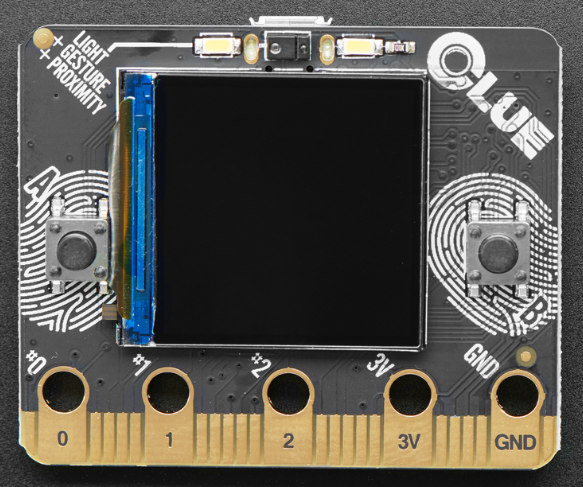
\includegraphics[scale=0.4]{Report/Images/ClueBoard.png}
    \caption{Adafruit CLUE board \cite{learnAdafruit}}
    \label{fig:adafruitClue}
\end{figure}

\subsection{CircuitPython}

CircuitPython is a programming language designed to be easy for beginners and experienced programmers alike to develop their own interactive projects. It adds hardware support to Python with libraries that allow you to code on low-cost microcontrollers and single board computers \cite{circuitpython}.

As Adafruit also supports the development of CircuitPython, it was the ideal programming language to code the experiments with. The boards using CircuitPython provide quick feedback which allow the programming of the experiments and libraries to be simple yet flexible.

\subsection{Kitronik Smart Greenhouse}

To run the experiments, the Kitronik Smart Greenhouse kit for BBC Micro:bit will be used. The CLUE board already has temperature and humidity sensors built in, alongside a handful of other useful components. The greenhouse kit provides an additional moisture sensor which can be connected to the board using crocodile clips, which are also provided. This will sit in the soil to regularly monitor the moisture levels. A motor and zip LEDs are also provided to allow control over how frequently the plant is watered and the level of light the plant is exposed to.

\begin{figure}[ht]
    \centering
    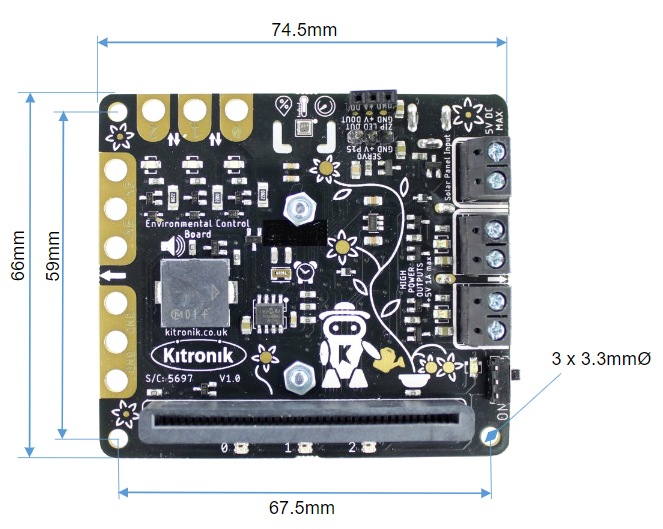
\includegraphics[scale=0.6]{Report/Images/KitronikBoard.png}
    \caption{Kitronik Environmental Control Board \cite{kitronikBoard}}
    \label{fig:KitronikBoard}
\end{figure}

\begin{figure}[ht]
    \centering
    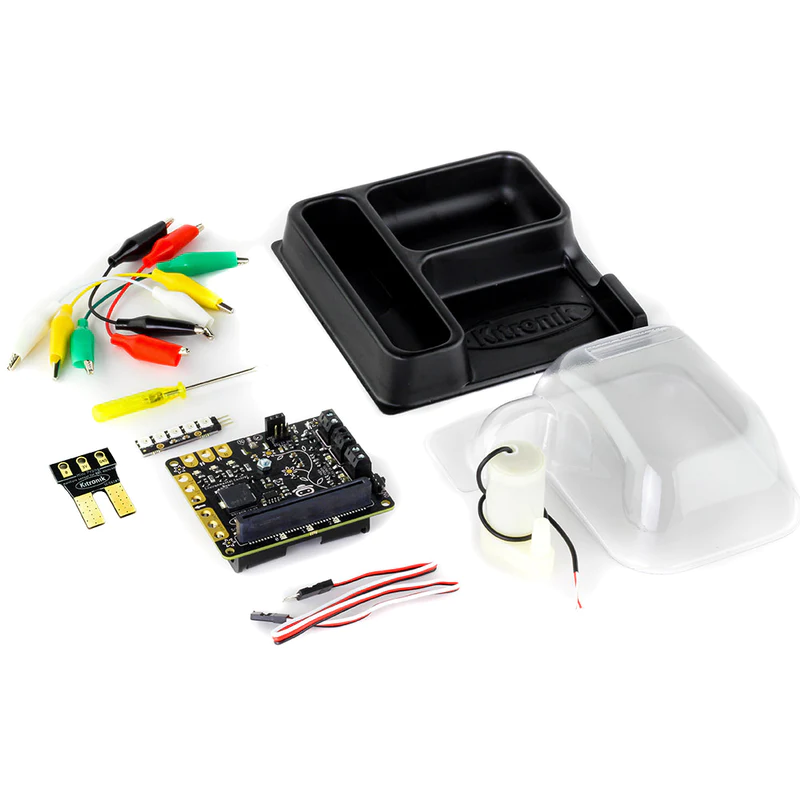
\includegraphics[scale=0.4]{Report/Images/KitronikGreenhouse.png}
    \caption{Kitronik Smart Greenhouse \cite{kitronikStore}}
    \label{fig:KitronikGreenhouse}
\end{figure}

% \chapter{Report Body}


\section{Section Heading}

\subsection{Subsection Heading}
\chapter{Requirements \& Specification}
% user stories should be somewhere

\section{Brief}

To see how different factors can affect the growth of plants, an experiment involving growing cress in varying environments will be run. A library will then be created in CircuitPython to make the creation of code (such as the experiments) for the Adafruit CLUE cleaner and easier to use.

\section{Experiments}

The Kitronik smart greenhouse will be the house to the experiments. Cress will be the seeds growing inside, and for each iteration of the experiment, the environment will be changed. The results for each round will be compared to the control run to see the difference in the final harvest. The purpose of this experiment is to show how changing parameters can affect the yield. This in turn shows that using machine learning can help us maximise yields by identifying the optimal levels of each variable.

\subsection{Variables}

The experiments that will be run in the Kitronik greenhouse will record the following:

\begin{itemize}
    \item Temperature
    \item Moisture levels of the soil
    \item Light (intensity and colour)
    \item Average height of cress strands
    \item Number of leaves
    \item Pictures of final growth for comparison
\end{itemize}

The first experiment will be a control, where there is only while light from the zip LEDs and a constant minimum moisture level of 0.5v. From there, the components that will be changed are the LEDs or the minimum moisture level. For the moisture level experiments, the minimum moisture levels (unit: voltage) will be set in the code using global constants. If the current water level falls below the given minimum, the motor will turn on to spray water briefly in order to bring the level back up. This should maintain a constant level and ideally show a difference in growth compared to the control run.

These experiments will run over the course of 6 weeks, giving each experiment one week to progress. At the same time every week, a record of the results will be taken and preparations for the next experiment will be made. This will include general maintenance of the greenhouse, replacing the water source, topping up soil if there is not sufficient and altering the code. At the end of the experimentation phase, we will compare the results to see if any difference was made by changing the variables. The aim is to see that light affects the cress growth differently to the moisture level.

\section{Library}

\subsection{Requirements}

To ensure the library includes everything we intend for it to do, writing up a list of requirements is essential. It helps visualise and prioritise functionality so developers do not get sidetracked into make unnecessary features or forget what's important to the client.

\subsubsection{User Stories}

\begin{itemize}
    \item As a user, I would like the library to be small in file size as the board has limited storage space.
    \item As a user, I would like to control the greenhouse equipment from my Adafruit CLUE.
    \item As a user, I would like the library to be easy to import.
    \item As a user, I would like the library to run fast and not slow down the code.
\end{itemize}

\subsubsection{Functional Requirements}
\begin{itemize}
    \item The library should allow the user to control the zip LEDs for the CLUE board.    
    \item The library should allow the user to control the motor to pump water connected to the CLUE board.
    \item The library should allow the user to get the moisture level of the environment the moisture sensor prongs are in.
    \item The library should allow the user to read the current temperature from the built-in thermometer.
\end{itemize}

\subsubsection{Non-Functional Requirements}

\begin{itemize}
    \item The functions for the library should be well documented.
    \item The library should not take up a lot or memory as the Adafruit CLUE board only has a storage space of about 2MB.
    \item The library should be easy to download and import.
    \item The library should be fast and not slow down the user's code.
\end{itemize}


\chapter{Design}

% Can be inconsistent with implementation but make sure you give reasons
% Choice of library and use case diagram

\section{Experiments}

Due to the time constraints, each experiment will run for six days. As cress is a fast growing herb, this should be sufficient time for the environment to have enough of an effect to show in its growth. The seventh day will then be used to take measurements of all the cress, clean the greenhouse and alter the code to create the next new growing conditions.

Although cress can be grown using hydroponics, the greenhouse will contain soil to keep the cress seeds in place. This also makes it easier to measure the moisture level as the moisture sensor can be placed in the soil and not straight into water which will continue to measure the same value. This soil will not be entirely changed for each round, instead topped up when necessary in order to maintain the same weight throughout each round. However, the water will be drained, cleaned and replaced to prevent growths, algae or mould appearing in the greenhouse and prevent it from getting caught in the water pump.

To keep all the experiments fair, they will all be using the same number of cress seeds. As the cress will be measured manually after the growing period, there shouldn't be an unreasonable amount, this also gives the cress space to grow and not interfere with each other. With space surrounding each seed, given the small space of the greenhouse, I plan to use 12 cress seeds per round of the experiment.

The dimensions taken by hand will be measured with a clear Oxford ruler and stored in an Excel spreadsheet. All the measurements taken by the greenhouse will be printed to the screen of the CLUE board and stored in a \textcolor{blue}{$.csv$} file. This file will be used to ensure the growing environment contained in the greenhouse is constant and fairly similar amongst all the rounds of the experiments (i.e. all the environment variables that may affect the growth of the cress). The Excel spreadsheet made by hand will then be used to create the graphs for evaluation and to make a final conclusion on the project. 

The experiments to run are as follows:

\begin{center}
\begin{tabular}{| c | c | c | c | c | c | c |} 
    \hline
    \textbf{Light} & White & No light & Red & Blue & White & White\\
    \hline
    \textbf{Moisture(v)} & 0.5 & 0.5 & 0.5 & 0.5 & 1 & 2\\
    \hline
\end{tabular}
\end{center}

The first experiment will be the control and will consist of a white light at maximum brightness with a constant moisture level of 0.5v. This will be used as a control run and all the other experiments will be compared to it to find which variables are affecting the growth in certain ways.

The following experiments change either the light colours or the moisture level. Experiments 2 - 4 maintain the same moisture level as the control but change the colour of the light. Experiments 5 and 6 maintain the same white light but with varying moisture levels. Using these experiments, we will be able to see how water and light can affect the growth of the cress.

\subsection{Hypothesis}

An article written about how different light qualities and intensities affect the growth and volatile compounds in plants state how their experiments conclude with higher light intensity resulting in increase of “root length, and leaf, shoot, root, and total weight” \cite{bayir2019plant}. It also concluded with red light showing highest leaf and total dry weight alongside a reduction in total monoterpenes, which are naturally occurring fragrant molecules with over 400 different structures \cite{ALCANTARA2011309}. Comparing this to blue light which showed a higher production in carvacrol which is a monoterpene often found in many aromatic plants used as spices such as oregano \cite{bayir2019plant}.

This leads to the hypothesis being that the control experiment with highest intensity of white light will have the longest stems and roots and therefore overall mass. Out of all the monochromatic lights, we will see if the red LED leads to the largest leaf span compared to the other colours. Unfortunately, it is difficult to obtain the necessary equipment to measure the levels of different monoterpenes in the cress. For this reason, we will still be running an experiment with blue light, not to measure the chemical compound levels, but to compare the leaf and other components to the white and red light experiments.

\section{Library}

\subsection{Design Pattern}

To deal with the number of different peripherals, the facade design pattern will be used. This is a structural design pattern that provides an interface to the library \cite{designPatterns}. The interface will hide the complexity and make creating experiments simple for beginners yet flexible enough for more confident users.

\begin{figure}[ht]
    \centering
    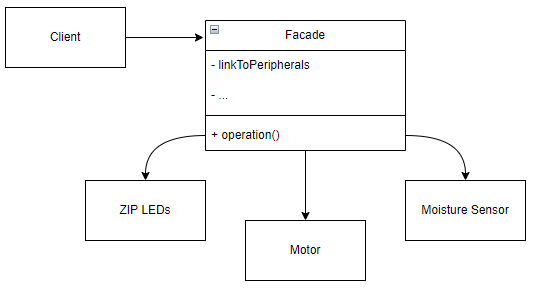
\includegraphics{Report/Images/facadePattern.png}
    \caption{Class diagram using a facade design pattern}
    \label{fig:classDiagram}
\end{figure}

The advantage of using a facade design pattern is that we can improve the usability of the library for the programmer.  However we want to avoid coupling the interface with too many classes. Often times, the main facade class can be linked with an additional facade to control other classes in the subsystem. \cite{designPatterns}

All the hardware that the greenhouse makes use of have their own class. These classes are then nested inside the facade class so that it can be used as an interface. This also allows the code to be extended without too much difficulty for new hardware and future refactorings. Having all these classes nested also allows the users to be able to simply import one library and have control over all the hardware needed for the greenhouse together without having a list of imports.

Each hardware component will have its corresponding class which will contain all the methods necessary to control it. For example, the class representing the zip LED will contain methods to change the colour of each LED and turn them on in any permutation the user wishes. The motor for the water pump may be turned on and off directly, or may be on for a specified time in seconds before being turned off automatically.

% testing go here
\chapter{Implementation}

For the development of this project, an iterative development cycle was used. As the running of the experiments are more passive than the development of the library, the environments for the experiments to run were created first. During the running of these experiments, I was then creating the code for the library and testing using a separate Adafruit CLUE I had at hand. I however did not have a spare Kitronik board, so on the seventh day of each experiment run, I would use the board for testing before running the next experiment for six days.

\section{Greenhouse Experiments}

\subsection{Understanding the Boards}

The initial part of developing the environments is to understand the hardware I was working with. The manual given with the Kitronik kit consisted of instructions for use with the Micro:bit, so understanding the different components on the Kitronik board, Adafruit CLUE and Micro:bit was necessary to find which pins correspond across the three. The pins on the Kitronik board connect to the hardware components and the board containing the code to control all the hardware components. The Kitronik board's pins are labelled using the same names as those on the Micro:bit.

\begin{figure}[H]
    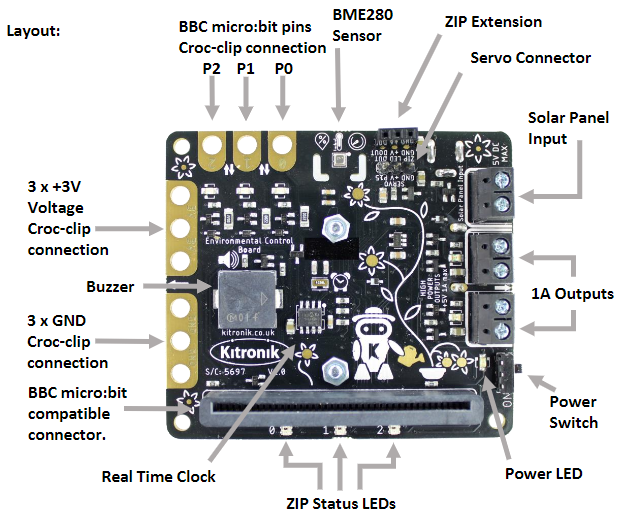
\includegraphics[scale=0.7]{Report/Images/KitronikBoardDiagram.png}
    \caption{Diagram of Kitronik Environmental Control board \cite{kitronikBoard}}
    \label{fig:KitronikDiagram}
\end{figure}

\begin{figure}[H]
    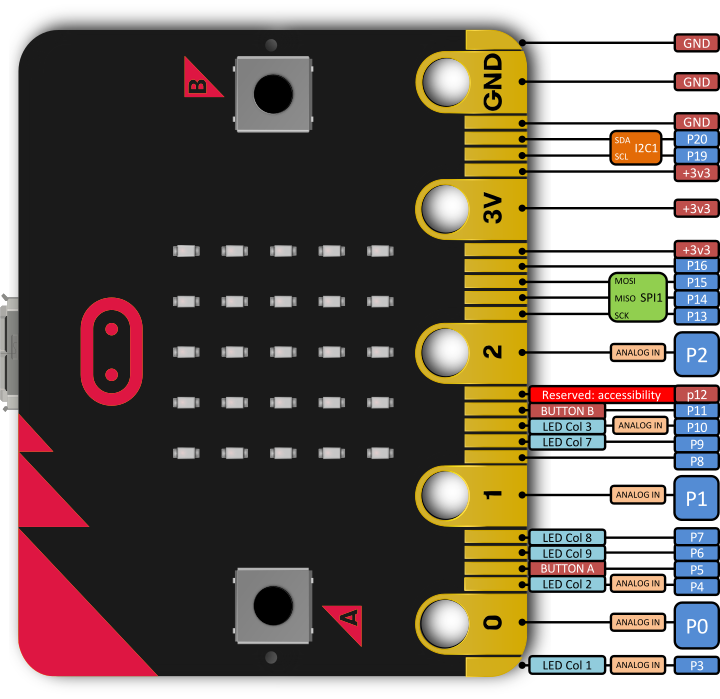
\includegraphics[scale=0.4]{Report/Images/MicrobitBoard.png}
    \caption{Diagram of Micro:bit board \cite{microbitDoc}}
    \label{fig:MicrobitBoard}
\end{figure}

\begin{figure}[H]
    \centering
    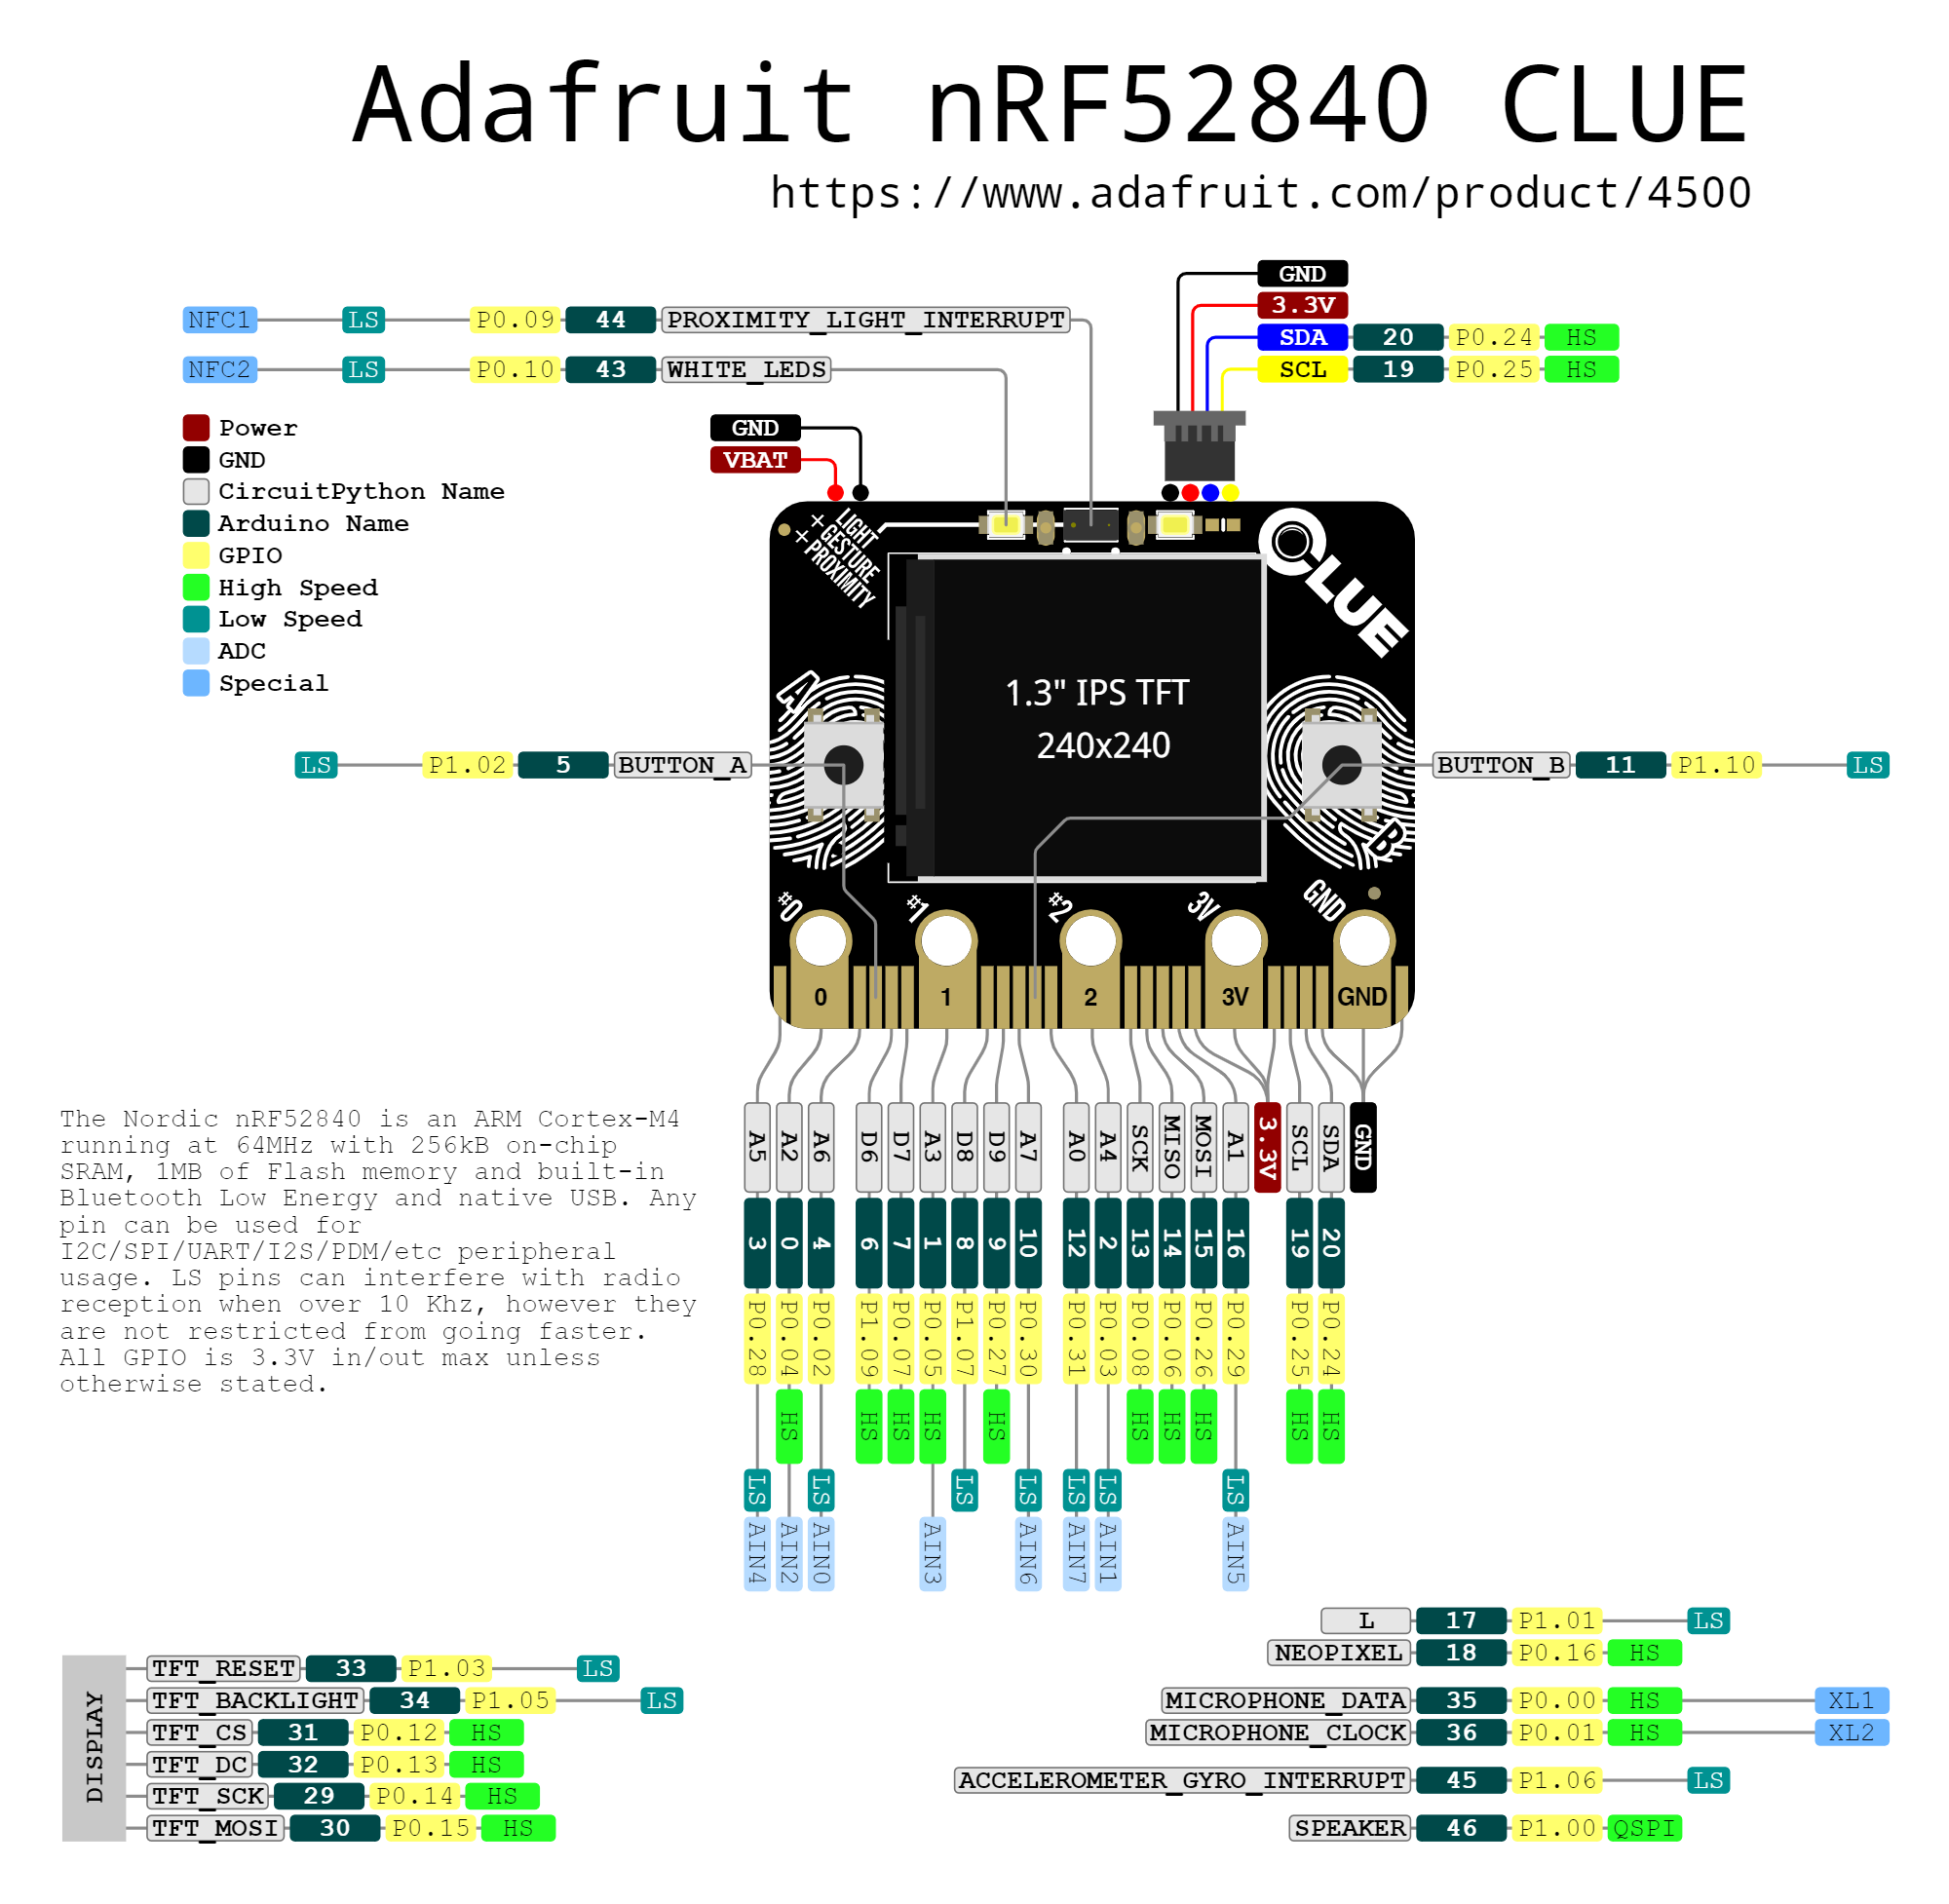
\includegraphics[scale=0.2]{Report/Images/ClueBoardDiagram.png}
    \caption{Diagram of Adafruit CLUE \cite{learnAdafruit}}
    \label{fig:CLUEDiagram}
\end{figure}

\begin{figure}[H]
    \centering
    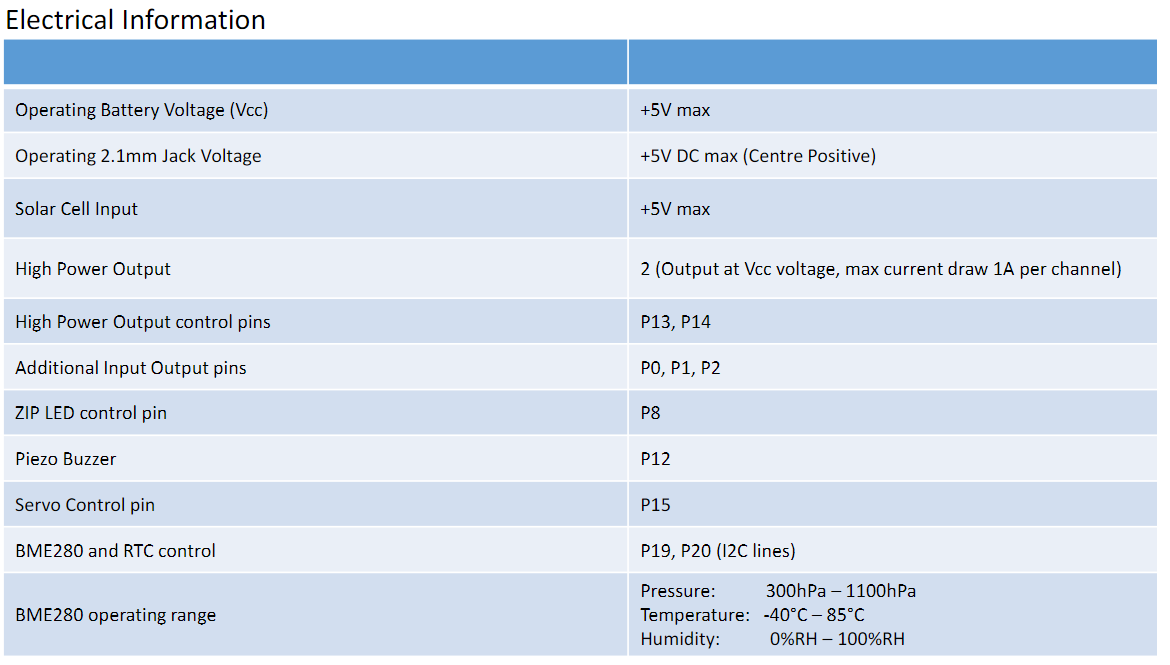
\includegraphics[scale=0.46]{Report/Images/KitronikInfoSheet.png}
    \caption{Environmental Control board datasheet \cite{kitronikBoard}}
    \label{fig:KitronikDatasheet}
\end{figure}

Using diagrams of the boards from their corresponding documentation plus the data sheet provided from the Kitronik kit, it was possible to see which pins on the Micro:bit match with the pins on the CLUE board without using trial and error:

\begin{center}
\begin{tabular}{| c | c | c | c | c | c | c | c |} 
    \hline
    \textbf{Micro:bit} & P0 & P1 & P2 & 3V & GND & P8 & P14\\
    \hline
    \textbf{CLUE} & A2 & A3 & A4 & 3.3V & GND & D8 & MISO\\
    \hline
\end{tabular}
\end{center}

On the Kitronik board, the pins P0, P1, P2 can all be used with crocodile clips to connect components such as the moisture sensor. The moisture sensor requires three crocodile clips: P0, 3V and GND. The ZIP LED has its own dedicated pins, which the datasheet specify uses P8. On the CLUE board this corresponds to the pin D8. Finally, the motor is a high voltage user and so is connected to pin P14 which corresponds to the pin MISO on the CLUE. The motor does not use crocodile clips, instead it is attached using two wires: positive and negative. These are stripped back slightly before being screwed into place (figure \ref{fig:KitronikDiagram}: the component labelled 1A outputs).

There are also a number of other built in sensors on both the Kitronik board and the CLUE:

\begin{itemize}
    \item Pressure sensor
    \vspace{-0.25cm}
    \item Thermometer
    \vspace{-0.25cm}
    \item Humidity sensor
    \vspace{-0.25cm}
    \item Light \& colour
    \vspace{-0.25cm}
    \item Sound etc.
\end{itemize}

\subsection{CircuitPython}

CircuitPython is a programming language made for using hardware. There are a number of libraries that make use of different components such as time, board and neopixel. For the experiments I will be using the following imports:

\begin{itemize}
    \item adafruit\_clue \cite{adafruitGit}
    \vspace{-0.25cm}
    \item rtc \cite{circPyDoc}
    \vspace{-0.25cm}
    \item time
    \vspace{-0.25cm}
    \item board
    \vspace{-0.25cm}
    \item neopixel \cite{neopixelGit}
    \vspace{-0.25cm}
    \item analogio
    \vspace{-0.25cm}
    \item digitalio
    \vspace{-0.25cm}
    \item microcontroller
\end{itemize}

The \textcolor{blue}{$adafruit\_clue$, $board$, $analogin$} and \textcolor{blue}{$digitalio$} imports allow me to specify which pins in the CLUE board to use when controlling the hardware.

e.g.
\begin{python}
    PIXEL_PIN = board.D8 
    analog_in = AnalogIn(board.A2)
    motor_pin = digitalio.DigitalInOut(board.MISO)
\end{python}

\textcolor{blue}{$rtc$} and \textcolor{blue}{$time$} are imported to control the time. In these experiments, time is used to hourly check if the plant needs watering, and to store the time and other parameters into a \textcolor{blue}{$.csv$} file. Lastly, \textcolor{blue}{$neopixel$} is the library used to control the ZIP LEDs on the top of the greenhouse.

To use all these libraries, I had to load them onto the CLUE board using a zip of up to date libraries on the CircuitPython website online \cite{circuitpython}. In the case of accidentally corrupting the board, this will need to be reloaded. And as the storage is only 2mb large, it is necessary to delete libraries that are not relevant to the project at hand. Especially as I will be storing data for the experiment on the board, there will need to be storage space as data will not be saved.

To load anything onto the board safely, you must be careful of not having any other power source connected to the CLUE board. It is also worth noting that nothing on the CLUE board should be updated directly. If a file (e.g. code) needs to be updated, then it is best to modify the code locally on your device, then replace the original file on the board.

\subsection{Storage}

Storing files generated by the code can be a little tricky for the Adafruit CLUE board. This is because it cannot allow multiple devices to simultaneously store files. Instead, the board has to specify only one device at a time can do so. 

First I had to create a \textcolor{blue}{$boot.py$} "which is executed before the USB connection is made" \cite{learnAdafruit}. The documentation for using the Adafruit CLUE supplied code to go into the file to set \textcolor{blue}{$readonly$} to \textcolor{blue}{$False$} on boot. The code in the boot file reads the input from pin D0. We can then use this as a switch for it we want to write via the code and or the USB. For my experiment, I set \textcolor{blue}{$readonly$} to \textcolor{blue}{$False$} when the pin is grounded, this way when the CLUE board is connected to the Kitronik board as part of the greenhouse, it will allow the code to write to file (which is necessary to log data).

\begin{python}[caption={boot.py}, captionpos=b]
    import board
    import digitalio
    import storage
    
    switch = digitalio.DigitalInOut(board.D0)
    switch.direction = digitalio.Direction.INPUT
    switch.pull = digitalio.Pull.UP

    storage.remount("/", switch.value)
\end{python}

Following the creation of \textcolor{blue}{$boot.py$}, learning how to write to file in code follows. This can be done by using \textcolor{blue}{$\textrm{open with}(x, y) \textrm{ as } z$} where \textcolor{blue}{$x$} is the file name, \textcolor{blue}{$y$} is the mode which determines whether what is being written to file appends the text or overwrites, and finally \textcolor{blue}{$z$} which is the variable name that will be used across the code when you are referring to the file. Nested in this block are methods \textcolor{blue}{$write$} and \textcolor{blue}{$flush$}  which are used on the file to log the data.

\begin{python}[caption={writing to file}, captionpos=b]
    try:
        with open("/experiment1.txt", "a") as fp:
            ... 
            fp.write("hello world")
            fp.flush()
            ...
    except OSError as e:
    ...
\end{python}

\subsection{Wiring the Board}

Setting up the greenhouse was a simple when using the instructional booklet that came with the set. First, the environmental board was wired up. This included using 3 sets of crocodile clips to connect the moisture sensor prongs. One wire was connected from the 0 pin on the moisture sensor to the 0 pin on the board. The second was connecting the 3v pins on the sensor to the board. Lastly, the GND pins on the sensor to the boards. The zip LEDs were connected to a tri-coloured set of wired that plugged straight into the designated area on the board. The motor for the water was a little more fiddly, requiring wire strippers to expose the inner wires in two thin cables. These were pushed into two small ports (negative and positive)) and then screwed into place.

Finally, the last set of crocodile clips were not used for any other components, but rather to allow the code to write to file. During the research phase, a \textcolor{blue}{$boot.py$} file was created to allow the code to write to file when a specified pin was grounded (the switch). So the final crocodile clip was connecting the 2 pin to GND so when the Adafruit CLUE board was inserted into the environmental board, the switch is on and the code is set to write mode.

One note to make about the equipment for the greenhouse is that the moisture sensor should not perform moisture check continuously, but rather occasionally as it can "promote rapid erosion of the electrodes".

% Add picture of the board's setup

\subsection{Creating the Environment}

% Mention how I created each environment
% The soil and whatnot that create the greenhouse
% Maybe mention the batteries? Make sure it's not too repetitive

\subsection{The Test Round}

The development of the code for the experiments consisted of using a number of constants throughout. This way, when developing the code for the next set of experiments, there only needed to be minor adjustments to the values of the constants. To ensure the code was working, I ran a test experiment. This was for a number of reasons such as making sure all the components were working, there wasn't too much of a delay for the time and the cress will grow a significant amount during that time.

Experiment number one (test) was with white light and a constant moisture level of 0.5v. Many unexpected events occurred during this week long time period. The greenhouse was kept in a small box to prevent other light sources affecting the course of the experiment, this was also to protect the greenhouse from physical damage such as item falling onto it and damaging the components. Within the first 24 hours of the project, a check was performed to find that the white light had turned red. The first assumption made was that the blue and green LED lights had broken, but it was decided that the project should keep running to find any other defects. A few hours later, the greenhouse was checked again to see that the screen of the Adafruit CLUE had turned off. Again another assumption was made that the screen was on standby, perhaps because nothing on the screen was changing. At the time, the code of the experiment did not print anything to screen, which was noted and to be changed for the next set of experiments. It was later found that the CLUE board did not record any information past the 6 hours that it remained awake (the \textcolor{blue}{$.csv$} file only contained 6 rows of information). On the sixth day of the experiment, the red light had fully died as well. This was the sign that the first experiment had ended. 

% Add pictures of the first experiment (20221230)

After concluding the first round had finished, it was time to measure all the different parts of the cress:

\begin{itemize}
    \item Leaf span
    \vspace{-0.25cm}
    \item Stem height
    \vspace{-0.25cm}
    \item Root length
\end{itemize}

All these measurements were taken taken by hand with a clear Oxford ruler and a clean wooden desk, and results stored in a spreadsheet for later use. For the first experiment, a spreadsheet was made to see the kind of data was being stored.

\begin{figure}[H]
    \centering
    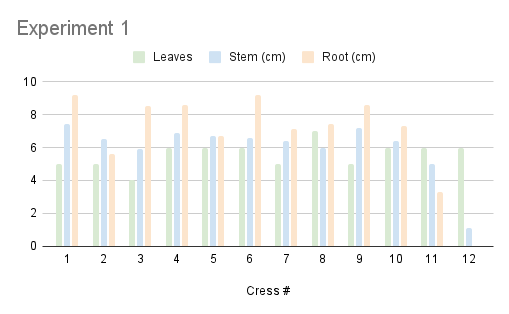
\includegraphics[scale=0.8]{Report/Images/Experiment1.png}
    \caption{Graph of results for experiment 1}
    \label{fig:experiment1}
\end{figure}

Although all the experiments' results will be concluded in the evaluation, it was important to check the results of the first test experiment immediately. In figure \ref{fig:experiment1}, we can conclude that the value for leaves did not vary by much cress to cress. Especially as the cress with fewer leaves often looked as if their leaves had yet to unfurl. In the spreadsheet, number of leaves was then changed to leaf span. For the last cress (cress number 12 in the diagram), the measurement of the stem and root were abnormally short. This anomaly was likely caused by the moisture sensory hindering its growth by being in the way. This then meant another change was to made to the experiments: the moisture sensor should be on the side of the tray of soil and out of the way of any of the seeds to prevent obstruction of growth.

Back to the running of the test experiment, it was also easy to conclude that the motor had been working fine as there were droplets of water found on the cress, and the soil was far from dry. However, it did seem that the soil was more wet than necessary as the \textcolor{blue}{$.csv$} file was returning high values for the moisture levels of the soil. This lead to another change in the code to pulse the motor on and off, giving the water time to spread through the soil and reach the moisture sensor before flooding the tray.

All that was left was the find the issue causing the LEDs to not work and the CLUE board to stop recording measurements. After testing all the hardware individually, it was discovered that the batteries needed replacing. This was a massive drawback in the board as there were at least 6 rounds of experiments to go and replacing the batteries every week is costly and bad for the environment. After a little more research into the board \cite{kitronikBoard}, there seemed to be a DC connected that could power the board straight from a socket. This allowed the board to be powered for the entirety of the project length without the need to purchasing and disposing of new AA batteries every week, as well as being a more reliable source of power. it is important to note that electricity often comes from fossil fuels which is not particularly eco-friendly either, but is better than disposing of lithium batteries at such a frequent rate.

\subsection{The Experiments}

The rest of the experiments performed without any other technical issues. The second experiment (the control experiment) was of white light and a moisture level of 0.5v. One seed did get lost in the soil (had not grown) and another barely germinated, having only a small stem visibly coming out of the seed with no root or leaves. The cress itself looked entirely different, with stronger stems and being able to hold themselves up. The green colour on the leaves and the stems was also a lot more vibrant compared to the first test experiment where the stems were white and the leaves a little paler.

% add picture of experiment 2 (20230106)
% Add the picture of all of them growing, the picture of it on the table and the picture of the seed

Experiment number three consisted of a constant blue light with a moisture level of 0.5v. The roots for this round were a lot larger than any of the other two, the longest reaching almost a foot long. They were extremely fine and hard to capture on camera. The leaves at the top were also a different shape, having a longer split in the stem before the leaves appeared. This made the averages of the leaf span a lot larger.

% Add picture (20230114)
% The leaf span and the ft long root

Experiment four used red light with the same 0.5v moisture. The roots were shorter and less fragile looking, with little fuzzy edges (unfortunately, the texture was too fine to pick up on camera). The leaves grew a little closer together and where more narrow compared to the long split in the blue light experiment.

% Add any pictures?

The no light experiment surprisingly grew taller than expected, yet the leaves had barely sprouted and the colour was more yellow than green. The stems grew very straight, likely as there was no light source to grow towards and the roots and stems were very similar lengths (compared to other experiments where there was often a big difference).

% pictures somewhere of the leaves being pale af

Experiment number six was for a lower moisture level in the soil set to 0.2v. This ended up different to the original plan of the last two experiment both being an increase in moisture. The reason being that 0.5v was alright leading to fairly moist soil for all the different light experiments. Instead, the final two experiments will consist of one lower moisture level and one higher. In this sixth round, the leaves where a little paler than the other rounds and a lot more delicate. The leaves did not spread very far and the roots grew a lot more than the other experiments. They did not have a longer average length than that of experiment 3, but rather, the roots where more than just one single strand like the other rounds. They took over the soil and were had to break apart for when it was time to measure them. Because of this, the root measurements may not be accurate as they may have ripped at the extraction stage. Another interesting thing to note is that the stems were more soft and unable to hold the weight of the cress as well.

% should be some images of the dry soil and the roots taking over

Lastly experiment number seven is with a white light and and moisture level set to 2.5v. The soil for the round was very wet, but considering cress can be grown using hydroponics, this should not be an issue. There are plenty of plants where soaking the seeds too long can cause them to drown. After six days, the cress had grown well, and wasn't much different than the control round which had less water. This shows that cress is fairly tolerant to high levels of water in their surrounding soil.


\section{Kitronik Library Development}

The idea behind creating a library for the Kitronik greenhouse kit is to make it easier for people using an Adafruit CLUE to create experiments and enjoy using the greenhouse. This single library will make code a lot easier and cleaner as there is less setting up and fewer imports to make. To implement this code, I will be creating a facade as an interface to all the imports needed. The interface itself will make use of the imports to set up the pins for all the hardware. This will require users to ensure they use the right pins for each component. To test this library does reduce complexity, I will be recreating the experiment code for the control round using the new library and comparing the code to the original version. Finally, I will be converting the file to \textcolor{blue}{$.mpy$} as all libraries on the CLUE board are of this format. \textcolor{blue}{$.mpy$} files contain bytecode of precompiled program from a Python source file \cite{micropython}. This can be done by using a program called \textcolor{blue}{$mpy-cross$}.

\subsection{Creating the Interface}

Creating the interface for the library initially including importing all the modules necessary for controlling the components that come with the greenhouse kits. This was then followed by the setting up of all the components. This includes specifying the pins for each piece of hardware, the number of lights on the zip LED and other small details needed to run code using these tools.

What came next was creating all the public functions that users can interact with. These were just basic controls for each hardware such as turning on and off the motor and getting values for the temperature and moisture level. For code that is designed for public use, documentation is a vital element of the interface. Each function required its own comment specifying its purpose, the parameters it takes and any return types. This needs to be concise yet understandable to beginners.

The more complex part of the code was simplifying the use of the LEDs. The ideal functionality is to allow the users to either control all of the lights simultaneously, or individually. This can be setting different colours to each pixel of light, or turning on only a few of them, but not all of them. More functionality that was added was timers for certain components. When creating the code for the experiments, the motor for the water was only used in short bursts, and not for one long period of time. Instead of the user importing the \textcolor{blue}{$time$} module, the user can call \textcolor{blue}{$motorTimer$} and specify a time in seconds for the motor to be turned on for. This was also added for the LED lights. Although simple, this functionality was added to the experiment's code after realising that the motor pumping water for a long period of time made the measurements for the moisture sensor less accurate as the water needed time to absorb into the soil and around the area the sensor was sitting. As for the LEDs, the timer can be used to create a cycle of night and day for the growing environment. 

\subsection{CookieCutter}

CookieCutter is a "command-line utility that creates projects from cookiecutters" \cite{cookiecutter}. It creates a template for Python libraries and can be used on Python version 3.7 and newer. To use, it must first be installed using the terminal (Linux in this case). Following this, the command to run CookieCutter is used. This returns a list of prompts that must be entered about the project. The text that is entered is used in the template comments regarding authors of the project, sponsored companies and more.

\begin{python}[caption={Installing CookieCutter on Linux}, captionpos=b]
    pip install cookiecutter
    cookiecutter gh:adafruit/cookiecutter-adafruit-circuitpython
\end{python}

Once CookieCutter has created the template file, all that is left is to copy and paste the library code that has been created into the\textcolor{blue}{$.py$} file that has been created. The purpose of this is to provide documentation on Github for other users. It includes a licenses folder for all the necessary Copyright files and example code files to understand how the library works.

\subsection{mpy-cross}

To use the library, it is preferred to have the \textcolor{blue}{$.py$} source code converted to a \textcolor{blue}{$.mpy$}. This is just as easy to import but is the precompiled version of the code. To create this package, \textcolor{blue}{$mpy-cross$} must first be downloaded \cite{libraryFileTypes} \cite{mpycrossDownloads}. The download is renamed to \textcolor{blue}{$mpy-cross$} and moved to the directory containing the Python source code. Ensuring the terminal is in the same directory as the \textcolor{blue}{$mpy-cross$} file and the source code, the following line must be entered into the terminal (where the path to the source code is changed accordingly).

\begin{python}
    ./mpy-cross path/to/your-library-file.py
\end{python}

To use the \textcolor{blue}{$.mpy$} file, it's as easy as copying it to your CIRCUITPY drive and importing the correct file name in the code. As it is bytecode, whitespace and comments are not included, which makes the file a lot smaller than using the Python source code file. As with any bytecode program, it does not need to be compiled again, and therefore uses less RAM on the board when compiling the entire program \cite{libraryFileTypes}.

\chapter{Machine Learning Model}

\section{Designing a Machine Learning Model}

\subsection{Different Machine Learning Models}

\subsection{Testing and Evaluating the Model}

% This could be moved to evaluation maybe?
% make more specific
Define the problem: Clearly define the problem you are trying to solve. In this case, the problem is to predict how different parameters affect plant growth.

Gather data: Collect data on various parameters that may affect plant growth, such as soil quality, temperature, humidity, sunlight, water, and fertilizers. The data should also include information on the growth of the plants, such as height, width, and yield.

Preprocess the data: Clean and preprocess the data to remove any missing values, outliers, or irrelevant features. Normalize the data to ensure that all features are on the same scale.

Split the data: Divide the data into training and testing sets. The training set is used to train the machine learning model, while the testing set is used to evaluate the performance of the model.

Choose a model: Choose a suitable machine learning model that can handle the given problem. In this case, a regression model, such as linear regression or decision tree regression, may be appropriate.

Train the model: Train the machine learning model using the training set. The model will learn the relationships between the different parameters and the plant growth.

Evaluate the model: Evaluate the performance of the model using the testing set. Use appropriate metrics, such as mean squared error or R-squared, to measure the accuracy of the model.

Optimize the model: If the model performance is not satisfactory, optimize the model by trying different hyperparameters or feature selection techniques.

Deploy the model: Once the model has been trained and optimized, deploy it in a production environment where it can be used to make predictions on new data.

Overall, designing a machine learning model for predicting how different parameters affect plant growth requires careful consideration of the problem, data collection, preprocessing, model selection, training, evaluation, and optimization.
\chapter{Legal, Social, Ethical and Professional Issues}
Your report should include a chapter with a reasoned discussion about legal, social ethical and professional issues within the context of your project problem. You should also demonstrate that you are aware of the regulations governing your project area and the Code of Conduct \& Code of Good Practice issued by the British Computer Society, and that you have applied their principles, where appropriate, as you carried out your project.

Talk about the kind of ppl that would use this research and how they may use it
good and bad uses

Talk about how it can affect societ for good or bad

other effects it can have on the world, research, agriculture and global warming

Could possibly mention moving to differnet planets and how growing stuff economically can benefit the planet and the astronauts 

\section{Section Heading}

\chapter{Results \& Evaluation}

\section{Experiment Results}
% Talk about how each experiment went?
% Talk about the experiments as a whole
% e.g. the graphs and what you would have learnt
% and what you would have changed for next time

The experimental phase finished over the course of roughly 8 weeks, including the creation of the code, running the experiments and redoing failed rounds. The evaluation of the experiments will be based on the hypothesis made in the Design chapter of the report. This section included how a papers reported different outcomes with different growing environments and how these can be applied to this project.

The hypothesis in question was based on red light producing plants with highest leaf and total dry weight. The other differences in growth were related to the chemical compounds produced, as there was not sufficient equipment provided to explore this further. Instead, measurements were made on the length of the different parts of the cress which correlates to the weight.

The \textcolor{blue}{$.csv$} file generated by the CLUE board in the greenhouse was used to ensure that the environment had stable conditions throughout the six day period. 
                              

\section{Library}   
% How did the library go?
% What have you learnt and what would you change for the next time


\chapter{Conclusion and Future Work}

% The project's conclusions should list the key things that have been learnt as a consequence of engaging in your project work. For example, ``The use of overloading in C++ provides a very elegant mechanism for transparent parallelisation of sequential programs'', or ``The overheads of linear-time n-body algorithms makes them computationally less efficient than $O(n \log n)$ algorithms for systems with less than 100000 particles''. Avoid tedious personal reflections like ``I learned a lot about C++ programming...'', or ``Simulating colliding galaxies can be real fun...''. It is common to finish the report by listing ways in which the project can be taken further. This might, for example, be a plan for turning a piece of software or hardware into a marketable product, or a set of ideas for possibly turning your project into an MPhil or PhD.


% in hindsight, would have been great to have a camera with software to measure the rate of growth, but this was realised too late and could not be done

In hindsight, the rate of growth would have been a great measurement to take for the machine learning model. Unfortunately this would require a camera with software to recognise the plant in order to record its length. This realisation came too late in the project, after the majority of the experiments had been run. Another thing that could have been changed in the experiment is including night and day cycles. This would pair well with tracking the growth rate as we can see how well the cress grew during the day and night periods.

To further this project, having different vegetation along side a much larger period of time would allow for for thorough research in the different components of growth. With a larger data set, the population will be more accurately represented in the machine learning model.                                                                                                                         




%%%%%%%%%%%%%%%%%%%%%%%%%%%%%%%%%
% References
%%%%%%%%%%%%%%%%%%%%%%%%%%%%%%%%%
\bibliographystyle{plain}
\bibliography{references}
\addcontentsline{toc}{section}{Bibliography}

%%%%%%%%%%%%%%%%%%%%%%%%%%%%%%%%%
% Appendices
%%%%%%%%%%%%%%%%%%%%%%%%%%%%%%%%%
\appendix
\chapter{Extra Information}
\section{Tables, proofs, graphs, test cases, ...}
The appendices contain information that is peripheral to the main body of the report. Information typically included in the Appendix are things like tables, proofs, graphs, test cases or any other material that would break up the theme of the text if it appeared in the body of the report. It is necessary to include your source code listings in an appendix that is separate from the body of your written report (see the information on Program Listings below).


\chapter{User Guide}
\section{Instructions}
You must provide an adequate user guide for your software. The guide should provide easily understood instructions on how to use your software. A particularly useful approach is to treat the user guide as a walk-through of a typical session, or set of sessions, which collectively display all of the features of your package. Technical details of how the package works are rarely required. Keep the guide concise and simple. The extensive use of diagrams, illustrating the package in action, can often be particularly helpful. The user guide is sometimes included as a chapter in the main body of the report, but is often better included in an appendix to the main report.

\chapter{Source Code}
\section{Instructions}
Complete source code listings must be submitted as an appendix to the report. The project source codes are usually spread out over several files/units. You should try to help the reader to navigate through your source code by providing a ``table of contents'' (titles of these files/units and one line descriptions). The first page of the program listings folder must contain the following statement certifying the work as your own: ``I verify that I am the sole author of the programs contained in this folder, except where explicitly stated to the contrary''. Your (typed) signature and the date should follow this statement.

All work on programs must stop once the code is submitted to KEATS. You are required to keep safely several copies of this version of the program and you must use one of these copies in the project examination. Your examiners may ask to see the last-modified dates of your program files, and may ask you to demonstrate that the program files you use in the project examination are identical to the program files you have uploaded to KEATS. Any attempt to demonstrate code that is not included in your submitted source listings is an attempt to cheat; any such attempt will be reported to the KCL Misconduct Committee.

\textbf{You may find it easier to firstly generate a PDF of your source code using a text editor and then merge it to the end of your report. There are many free tools available that allow you to merge PDF files.}


\end{document}